\documentclass{paper}
\usepackage{times}
\usepackage{geometry}
\geometry{letterpaper, portrait, margin=1in}
\usepackage[utf8]{inputenc}
\usepackage{enumitem,amssymb}
\usepackage{ragged2e}
\usepackage{physics}

\usepackage{caption}
\usepackage{hyperref}
\usepackage{url}

\usepackage{graphicx}
\usepackage{epstopdf}
\graphicspath{{data/cos-w1}}

\usepackage{biblatex}
\bibliography{refs}

\title{cos-w1 tasks}
\author{ariahayd}
\date{1 February 2022}

\begin{document} 

\maketitle

\begin{enumerate}
    \item % 1.
      Where the number density $n$ in the star cluster declines as 
      $1/r$, the the total number of objects with a measurable flux 
      $f$ within a radius $r$ to an observer at the center of the cluster 
      is given, with the differential in $r$, by: 

      \begin{equation}
        N = \frac{4}{3} \pi r^3 \left( \frac{n}{r} \right) \implies 
        \dv{N}{r} = \frac{8}{3} \pi r n
      \end{equation}

      The cluster is populated by stars assumed to have uniform luminosity, 
      so the flux $f$ from each source and differential along the radius is:

      \begin{equation}
        f = \frac{L}{4 \pi r^2} \implies \dv{f}{r} = -\frac{L}{2 \pi r^3}
      \end{equation}

      Dividing $(1)$ by $(2)$ yields:
      \[ \dv{N}{f} = -\frac{16 \pi^2 r^4 n }{3 L} \propto r^4 \]

      Because of $(2)$, $r^2 \propto f^{-1}$, which can be substituted into 
      the proportionality to remove dependence on $r$ and to fix $\alpha$:
      \[  \dv{N}{f} \propto f^{-2} = f^{\alpha} \implies \alpha = -2 \]

      Counts are analyzed in logarithmic bins of flux, so it is necessary to
      substitute $\frac{1}{f}\dd{f} = \dd{(\ln{f})}$ into the expression 
      relating count and flux:
      \[ f \dv{N}{f} = \dv{N}{\ln{f}}
      = \mathcal{C} f^{\alpha + 1} = \mathcal{C} f^{-1} \]

      Taking the log of both sides and substitute $\alpha$,
      \[ \log{\left(\dv{N}{\ln{f}}\right)} = (\alpha + 1)\log{f} + \mathcal{C}
      = -\log{f} + \mathcal{C} \]

      In this model, the log binning of the number count of stars in the
      cluster is linearly proportional to the log of flux measured by
      the observer. This relationship is due to the $1/r$ decline in number
      density $n$ around the observer, and if they were to determine this
      relationship through measurements, they would be able to discern the
      inhomogeneity of their surroundings. The distribution of stars in the
      cluster is nonhomogeneous, would be isotropic from the perspective of 
      the observer, but not isotropic generally.

  \pagebreak \item % 2.
    \begin{enumerate}
      \item
        The NRAO VLA Sky Survey (NVSS) measured, over four years, the 1.4 
        GHz flux from field ``snapshot'' views of the sky north of -40, 
        stitched together to make 4°×4° patches with polarization data along 
        the third dimension. A catalog of 2e6 discrete source features with 
        flux density $S$ greater than 2.5 mJy were extracted from the cubes. 
        Measurement error in the position in the sky of point sources varies 
        with the measured irradiance, from 7" uncertainty at the lower limit 
        to less than 1" in the bin of highest $S$. The catalog derived from
        this data set includes ``radio galaxies and quasars\ldots ultraluminous 
        starburst galaxies even at cosmological distances, plus statistically 
        useful numbers of nearby ``normal'' galaxies, low-luminosity 
        active galactic nuclei (AGNs), Galactic planetary nebulae, pulsars, 
        and stars.''\cite{Condon_1998}

      \item
        The Two Micron All Sky Survey (2MASS) recorded data in three 
        near-infrared bandpasses in the J, H, and Ks bands, simultaneously. 
        The survey covered nearly the entire sky from two ground-based 1.3m 
        diameter telescopes in both the northern and southern hemispheres of
        Earth over four years. Integrating the flux from each point over 7.8s 
        allowed for detecting sources of minimum magnitude 15.8, 15.1, and 
        14.3 in each of band respectively.\cite{Skrutskie_2006}

      \item
        Using the 2MASS data as input to select targets in the Ks band, the
        2MASS Redshift Survey (2MRS) mapped the distributions of nearby
        galaxies in 3D space using spectroscopy to determine the redshift, 
        and redshift as a proxy for distance. This survey started with a 
        sample of 44,599 2MASS galaxies with magnitude in the Ks band  
        brighter than 11.75 outside of the galactic plane by 5° (and by 8°
        near the center). The research team measured spectroscopy for 11,000
        samples to complete 97.6\% of the samples in the original data set at 
        the point of relase, covering 91\% of the sky.\cite{Huchra_2012}

    \end{enumerate}

  \pagebreak \item % 3.
    \begin{enumerate}
      \item
        A subset of NVSS data in the range from a minimum of 2.8 mJy to a
        maximum of 5000 mJy represents 84\% of the sample. This line fit to 
        the binned curve of this subset has a slope of -1.1, as shown in 
        Figure \ref{fig:nvss-bins}. This slope matches the model of an 
        inhomogeneous density as predicted in (1).  The slope of a linear fit 
        to the bins would vary slightly across the distribution, but only 
        significantly if only the extremes of data set were sampled.  Could 
        the slope fitting the model in (1) be due to cosmological redshift of 
        AGN radio sources making the density distribution appear closer to a 
        $1/r$ dropoff? This result would mean that the luminosity of 
        measureable redshifted sources is reduced by a factor of $1/r$ which 
        fits with the expansion model in which energy density of radiation 
        declines as $r^{-4}$.

        \begin{figure}[!htb]
          \includegraphics[width=\linewidth]{nvss.eps}
          \caption{NVSS samples binned by irradiance, both scales in log}
          \label{fig:nvss-bins}
        \end{figure}

      \item
        A subset of 2MASX data between 15 mag at the dimmest and 8 mag at the
        brightest fits a line of slope 0.55, which is close to the predicted
        value of 0.6 for a homogenous density model in the magnitude scale.
        This subset represents 65\% of the total data set. This analysis
        is of J band signals. See Figure \ref{fig:2masx-bins}.

        \begin{figure}[!htb]
          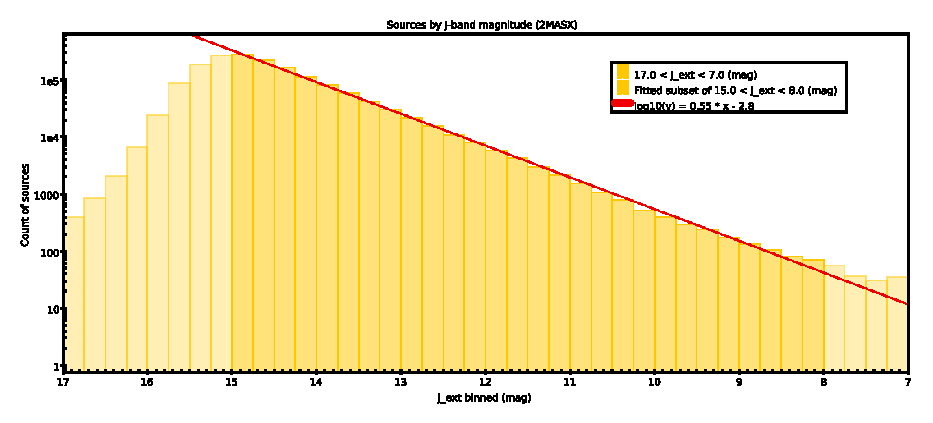
\includegraphics[width=\linewidth]{2masx.eps}
          \caption{2MASX samples binned by mag J band, count in log}
          \label{fig:2masx-bins}
        \end{figure}

      \item
        A similar analysis of a subset of data from the 2MRS data set, 
        though a subset that represents a greater fraction of the overall 
        data set than was selected for the 2MASX analysis, shows the same
        value for slope (0.55 for a model that predicts 0.6). This subset
        represented 88\% of the data set and spans 11.5 mag to 7.0 mag in the
        K band. See Figure \ref{fig:2mrs-bins}

        \begin{figure}[!htb]
          \includegraphics[width=\linewidth]{2mrs.eps}
          \caption{2MRS samples binned by mag K band, count in log}
          \label{fig:2mrs-bins}
        \end{figure}

    \end{enumerate}
  \pagebreak \item % 4.
    \begin{enumerate}
      \item
        The 2MRS catalog limited to sources with $cz < 8500 km/s$ is shown in
        Figure \ref{fig:2mrs-czg} in a projection oriented to the galactic
        plane. This makes up 50\% of the sources in the data set. The 
        $cz$ value is measure through spectroscopy of each source and can be
        used as a proxy for distance given the assumption that recession
        velocities increase with distance.

        Limiting to this subset reveals some filamentary structure that runs 
        across and it divided by the void in the middle of the projection. 
        This void is do to extinction in the source light by the Milky Way 
        band.

        \begin{figure}[!htb]
          \includegraphics[width=\linewidth]{2mrs-czg.eps}
          \caption{Nearest 50\% of 2MRS sources in Aitoff projection 
            oriented to the galactic plane, as determined by $cz$}
          \label{fig:2mrs-czg}
        \end{figure}
    
      \item
        Figure \ref{fig:2mrs-czsg} is the 2MRS catalog limited to the sources 
        with $cz$ determined to be less than 8500 km/s, making up the nearest
        50\% of source objects. 

        In this view, the structures are not divided by the plane of the
        Milky Way, and appear less filamentary and more globular.
        \begin{figure}[!htb]
          \includegraphics[width=\linewidth]{2mrs-czsg.eps}
          \caption{Nearest 50\% of 2MRS sources in Aitoff projection 
            oriented to the supergalactic local group plane, as determined 
            by $cz$}
          \label{fig:2mrs-czsg}
        \end{figure}
    \end{enumerate}
\end{enumerate}

This paper is available publicly.\cite{Hayden_Cosmology_Source_Repo}

\pagebreak
\printbibliography

\end{document}

